\documentclass[
	12pt,				% tamanho da fonte
	openright,			% capítulos começam em pág ímpar (insere página vazia caso preciso)
	oneside,			% para impressão em recto e verso. Oposto a oneside
	a4paper,			% tamanho do papel. 
	english,			% idioma adicional para hifenização
	french,				% idioma adicional para hifenização
	spanish,			% idioma adicional para hifenização
	brazil				% o último idioma é o principal do documento
	]{abntex2}

\usepackage{lmodern}			% Usa a fonte Latin Modern			
\usepackage[T1]{fontenc}		% Selecao de codigos de fonte.
\usepackage[utf8]{inputenc}		% Codificacao do documento (conversão automática dos acentos)
\usepackage{indentfirst}		% Indenta o primeiro parágrafo de cada seção.
\usepackage{color}				% Controle das cores
\usepackage{graphicx}			% Inclusão de gráficos
\usepackage{microtype} 			% para melhorias de justificação
\usepackage{transparent}
\usepackage{eso-pic}
\usepackage{amsthm,amsfonts}
\usepackage{float}
\usepackage{multirow}
\usepackage[table,xcdraw]{xcolor}
\usepackage{lipsum}				% para geração de dummy text
\usepackage[brazilian,hyperpageref]{backref}	 % Paginas com as citações na bibl
\usepackage[alf]{abntex2cite}	% Citações padrão ABNT
\usepackage{xcolor}
\definecolor{verde}{rgb}{0,0.5,0}
\usepackage{listings}
\lstset{
  language=C++,
  basicstyle=\ttfamily\small,
  keywordstyle=\color{blue},
  stringstyle=\color{verde},
  commentstyle=\color{red},
  extendedchars=true,
  showspaces=false,
  showstringspaces=false,
  numbers=left,
  numberstyle=\tiny,
  breaklines=true,
  backgroundcolor=\color{green!10},
  breakautoindent=true,
  captionpos=b,
  xleftmargin=0pt,
}


\titulo{Trabalho sobre \\Sistemas de Controle}
\autor{Gabriel R. Munhoz 106802\\João Vítor Batistão 108074}
\local{Maringá, PR}
\data{13.11.2021}
\orientador{}
\coorientador{}
\instituicao{%
  Universidade Estadual de Maringá - UEM
  \par
  Departamento de Engenharia de Produção - DEP}
\tipotrabalho{Tese (Doutorado)}
\preambulo{}

\definecolor{blue}{RGB}{41,5,195}

\makeatletter
\hypersetup{
     	%pagebackref=true,
		pdftitle={\@title}, 
		pdfauthor={\@author},
    	pdfsubject={\imprimirpreambulo},
	    pdfcreator={LaTeX with abnTeX2},
		pdfkeywords={abnt}{latex}{abntex}{abntex2}{trabalho acadêmico}, 
		colorlinks=true,       		% false: boxed links; true: colored links
    	linkcolor=blue,          	% color of internal links
    	citecolor=blue,        		% color of links to bibliography
    	filecolor=magenta,      		% color of file links
		urlcolor=blue,
		bookmarksdepth=4
}

\setlength{\parindent}{1.3cm}

\setlength{\parskip}{0.2cm}  % tente também \onelineskip

\makeindex

\usepackage{fancyhdr}
\fancyhead{}
\fancyfoot{}
\lhead{Trabalho sobre Sistemas de Controle}
\rhead{\thepage}

\AddToShipoutPicture{
\put(0,0){
\parbox[b][\paperheight]{\paperwidth}{%
\vfill
\centering
{\transparent{0.1}
\includegraphics[scale=1.4]{../../Pictures/LogoUEM.jpg}       }%
\vfill}}}

%\graphicspath{{../Pictures}}
\begin{document}

\begin{minipage}[c][0cm][c]{0cm} % a primeira minipágina tem uma altura de 1.5cm e uma largura de 3cm.

\centering


\includegraphics[scale=0.45]{../../Pictures/uem-modelo-04.png}  
\end{minipage}

\selectlanguage{brazil}

\frenchspacing 

% \pretextual

\imprimircapa


% ---
% RESUMOS
% ---

%\setlength{\absparsep}{18pt} % ajusta o espaçamento dos parágrafos do resumo
%\begin{resumo}
 
 
% \textbf{Palavras-chave}: latex. abntex. editoração de texto.
%\end{resumo}


% ---
% inserir o sumario
% ---
\pdfbookmark[0]{\contentsname}{toc}
\tableofcontents*
\cleardoublepage

% ----------------------------------------------------------
% ELEMENTOS TEXTUAIS
% ----------------------------------------------------------
\textual

\chapter{Introdução}
\pagestyle{fancy}

O trabalho realizado tem foco no estudo de um sistema de um tanque agitado com duas correntes de entrada, sendo uma de água pura e outra de solução aquosa de hidróxido de sódio, conforme a Figura \ref{Modelo do Tanque}. Será realizada a classificação das variáveis desse sistema, o desenvolvimento das funções de transferência do modelo do processo, a estruturação de um diagrama de blocos e a apresentação da dinâmica do processo utilizando o software Xcos.

\begin{figure}[!h]
\centering
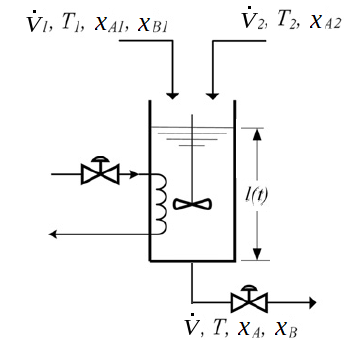
\includegraphics[scale=0.6]{1a.png} 
\caption{Modelo do Tanque}
\label{Modelo do Tanque}
\end{figure}

A modelagem do sistema acima resultou no levantamento das seguintes hipóteses e equações:

\begin{itemize}
\item Mistura perfeita;
\item Propriedades físicas constantes;
\item Calor de mistura desprezível;
\item Tanque isolado e $\dot{W}_{s}$ é desprezível.
\end{itemize}

Balanço de Massa Global:
\begin{equation}
\frac{dl}{dt}=\frac{(\dot{V}_{1}+\dot{V}_{2}-\dot{V})}{A}
\end{equation}

Balanço de Massa para Componente A:
\begin{equation}
Al\frac{dx_{A}}{dt}=\dot{V}_{1}(x_{A,1}-x_{A})+\dot{V}_{2}(x_{A,2}-x_{A})
\end{equation}

Balanço de Massa para Componente B:
\begin{equation}
Al\frac{dx_{B}}{dt}=\dot{V}_{1}(x_{B,1}-x_{B})+\dot{V}_{2}(x_{B,2}-x_{B})
\end{equation}

Balanço de Energia:
\begin{equation}
\overline{\rho}\overline{C}_{p}Al\frac{dT}{dt}=\overline{\rho}\overline{C}_{p}\dot{V}_{1}(T_{1}-T)+\overline{\rho}\overline{C}_{p}\dot{V}_{2}(T_{2}-T)+\dot{Q}
\end{equation}

Com essa modelagem é possível classificar as variáveis do sistema e realizar os cálculos das funções de transferência para que possa ser verificado o impacto que cada variável de entrada possui no controle das variáveis de saída.

\newpage
\chapter{Classificação de variáveis}
\pagestyle{fancy}

As variáveis do sistema podem ser classificadas como parâmetros, variáveis de entrada e variáveis de saída. A primeira classificação faz menção as variáveis que são estabelecidas como constantes do sistema, ou seja, durante as simulações elas sempre se mantém as mesmas. As variáveis de entrada e saída no entanto, são aquelas que se alteram durante o percorrer do tempo e se diferem por serem variáveis das correntes de entrada ou da de saída.

\textbf{Parâmetros:}
\begin{itemize}
\item Área do tanque (A);
\item Calor ($\dot{Q}$);
\item Densidade do líquido ($\rho$);
\item Calor específico do líquido ($C_{p}$);
\end{itemize}

\textbf{Variáveis de Entrada:}
\begin{itemize}
\item Temperatura da corrente 1 ($T_{1}$);
\item Temperatura da corrente 2 ($T_{2}$);
\item Composição de água na corrente 1 ($x_{a,1}$);
\item Composição de hidróxido de sódio na corrente 1 ($x_{b,1}$);
\item Composição de água na corrente 2 ($x_{a,2}$);
\item Composição de hidróxido de sódio na corrente 2 ($x_{b,2}$);
\item Vazão de entrada da corrente 1 ($\dot{V}_{1}$);
\item Vazão de entrada da corrente 2 ($\dot{V}_{2}$);
\end{itemize}

\textbf{Variáveis de Saída:}
\begin{itemize}
\item Altura do tanque (l);
\item Vazão de saída do tanque ($\dot{V}$);
\item Composição de água na corrente de saída ($x_{a}$);
\item Composição de hidróxido de sódio na corrente de saída ($x_{b}$);
\item Temperatura da corrente de saída (T);
\end{itemize}

As variáveis de entrada são classificadas também como sendo variáveis de manipulação, já que por meio do seu manuseio é possível manipular as variáveis de saída do sistema. Essas últimas também podem ser chamadas de variáveis controladas pelo mesmo motivo. 

Contudo, é importante entender que nem toda variável de entrada consegue manipular qualquer variável de saída, pois boa parte dessas variáveis se relacionam de maneira independente, e quando existe essa independência apenas com uma variável de entrada igual a de saída que é possível realizar manipulações. Como por exemplo a vazão, mesmo alterando a temperatura ou a concentração das correntes de entrada não é possível alterar a vazão de saída a menos que se altere a vazão de uma das correntes de entrada.

Em sistemas mais complexos é difícil entender o quanto a mudança de uma variável de manipulação implica na alteração de uma variável de controle. Para isso existem as funções de transferência, que conseguem definir o quanto uma variável depende da outra.

\newpage
\chapter{Funções de Transferência}
\pagestyle{fancy}

As funções de transferência são funções que como já mencionadas anteriormente são capazes de demonstrar o quanto uma variável é dependente de outra. Esses funções são calculadas por meio da seguinte fórmula:

\begin{equation}
G(s) = \frac{\mathcal{L}[saída]}{\mathcal{L}[entrada]}
\end{equation}

Variáveis de desvio:
\begin{eqnarray}
x'_{a,1} &=& x_{a,1} - \overline{x}\\
x'_{a} &=& x_{a} - \overline{x_{a}}\\
\dot{V'}_{1} &=& \dot{V'}_{1} - \overline{\dot{V}_{1}}\\
\dot{V'}_{2} &=& \dot{V'}_{2} - \overline{\dot{V}_{2}}
\end{eqnarray}

Partindo do Balanço de Massa para o Componente A (1.2) e das equações de desvio acima listadas é possível realizar a linearização da mesma, resultado na seguinte equação:

\begin{equation}
Al\frac{dx'_{A}}{dt} = -(\overline{\dot{V}_{1}}+\overline{\dot{V}_{2}})x'_{a} + \overline{\dot{V}_{1}}x'_{a,1} + (\overline{x_{a,1}}-overline{x_{a}})\dot{V'}_{1} + (\overline{x_{a,2}}-\overline{x_{a}})\dot{V'}_{2}
\end{equation}

Aplicando La Place na equação 3.6 tem-se:

\begin{equation}
Alx_{a}(s) = -(\overline{\dot{V}_{1}}+\overline{\dot{V}_{2}})x_{a}(s) + \overline{\dot{V}_{1}}x_{a,1}(s) + (\overline{x_{a,1}}-overline{x_{a}})\dot{V}_{1}(s) + (\overline{x_{a,2}}-\overline{x_{a}})\dot{V}_{2}(s)
\end{equation}

Para compreender melhor o sistema é importante o cálculo das seguintes variáveis de saída: concentração do componente 'a' ($x_{a}$) e a altura (l), em relação as seguintes variáveis de entrada: vazão da corrente 1 ($\dot{V}_{1}$), vazão da corrente 2 ($\dot{V}_{2}$) e conentração do componente 'a' na corrente 1 ($x_{a,1}$).

\begin{eqnarray}
\frac{l(s)}{V_{1}(s)} \quad
\frac{l(s)}{V_{2}(s)} \quad
\frac{x_{A}(s)}{V_{1}(s)} \quad
\frac{x_{A}(s)}{x_{a,1}(s)} \quad
\frac{x_{A}(s)}{V_{2}(s)}
\end{eqnarray}

Assim com a equação 3.7 que é uma função de transferência pode-se com manipulações matemáticas encontrar os valores das relações acima, e com esses valores é possível realizar a manipulação no software Xcos.


\newpage
\chapter{Diagrama de Blocos}
\pagestyle{fancy}

Para melhor entendimento do fluxo de informações que ocorre no sistema o diagrama de blocos é muito importante, pois melhora a visualização do sistema e facilita a aplicação em softwares de simulação.

\begin{figure}[!h]
\centering
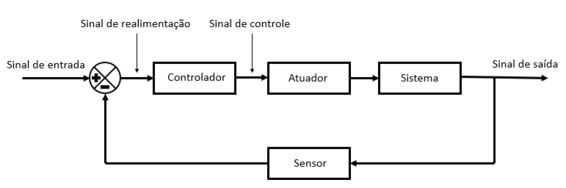
\includegraphics[scale=0.6]{DiagramaBlocos.jpeg} 
\caption{Diagrama de Blocos}
\label{Diagrama}
\end{figure}

Nesse diagrama é possível notar que o sistema que será estudado é um sistema de malha fechada, visto que há um feedback do sensor que pode manipular alguma variável de entrada. Já em casos onde o sistema possui uma malha aberta não há o controle de uma variável por meio dos dados do sensor, esses dados são apenas utilizados para leitura, no diagrama de blocos isso seria fácil de identificar, se o sistema fosse de malha aberta não ocorreria a ligação do sensor com o controlador.

\newpage
\chapter{Dinâmica do Processo - Software Xcos}
\pagestyle{fancy}

\newpage
\chapter{Simbologia}
\pagestyle{fancy}

\begin{itemize}
\item Q - Calor - Unidade: kJ;
\item $\dot{Q}$ - Taxa de calor - Unidade: kW;
\item $C_{p}$ - Calor específico - Unidade: kJ/(kg*K);
\item $\rho$ - Densidade - Unidade: $kg/m^{3}$;
\item $x$ - Concentração - Unidade: pu;
\item V - Volume - Unidade: $m^{3}$;
\item $\dot{V}$ - Vazão do líquido - Unidade: $m^{3}/s$;
\item A - Área - Unidade: $m^{2}$;
\item l - Altura - Unidade: m;
\item T - Temperatura - Unidade: K;
\item $E_{T}$ - Energia total - Unidade: kJ;
\item $E_{p}$ - Energia potencial - Unidade: kJ;
\item $E_{k}$ - Energia cinética - Unidade: kJ;
\item U - Energia interna - Unidade: kJ;
\item H - Entalpia - Unidade: kJ/mol;
\item m - Massa - Unidade: kg;
\item $\dot{M}$ - Vazão mássica - Unidade: kg/s;
\end{itemize}

\newpage
\postextual


\bibliography{referencia}


\end{document}
